%%%%%
%%Title: HiPi+Bus V0.2 Chapter 6
%%Creator: Ando Ki
%%CreationDate: April 1992
%%FileName: sec5
%%RelatedFile: ch6
%%%%%
\section{인터럽트버스의 시간규격}
%
\subsection{IBSYNC* 신호의 시간규격}
IBSYNC* 신호는
백플레인에 나타나는 버스클럭의 하강점에서 $TP^{IBSYNC}_0$후에
안정된 신호를 래치할 수 있도록 셋업시간으로 $TP^{IBSYNC}_2$을
홀드시간으로 $TP^{IBSYNC}_3$를 보장해야 한다.
IBSYNC* 신호를 ``거짓(high voltage level)''로 하기 위해서는
구동을 멈추어야 하는데 이때 다음 신호에 영향을 주지 못하도록 $TP^{IBSYNC}_4$을
보장해야 한다. 여러 버스 사이클 동안 구동하는 경우, $TP^{IBSYNC}_1$은
처음 사이클에서, $TP^{IBSYNC}_4$는 마지막 사이클에서만 지키면 된다.
%\documentstyle[a4]{hbook}
%\begin{document}
%
\begin{table}[htbp]
\caption{IBSYNC* 신호의 시간규격 요약}\label{table:ibsync-time}
   \begin{center}
   \begin{tabular}{|l|l|r|r|r|} \hline
	timing parameter & name & min & typical & max \\ \hline \hline
	$TP^{BCLK}_0$   & BCLK* cycle time & 59 & 60 & 61 \\ \hline
	$TP^{IBSYNC}_0$  & IBSYNC* latch point & 38 & 40 & 42 \\ \hline
	$TP^{IBSYNC}_1$  & bus propagation time & - & - & 20 \\ \hline
	$TP^{IBSYNC}_2$  & IBSYNC* setup time & 10 & - & - \\ \hline
	$TP^{IBSYNC}_3$  & IBSYNC* hold time & 5 & - & - \\ \hline
	$TP^{IBSYNC}_4$  & IBSYNC* guard time & 10 & - & - \\ \hline
   \end{tabular}
   \end{center}
\end{table}
%
%\end{document}

\begin{figure}[htb]
    \centerline{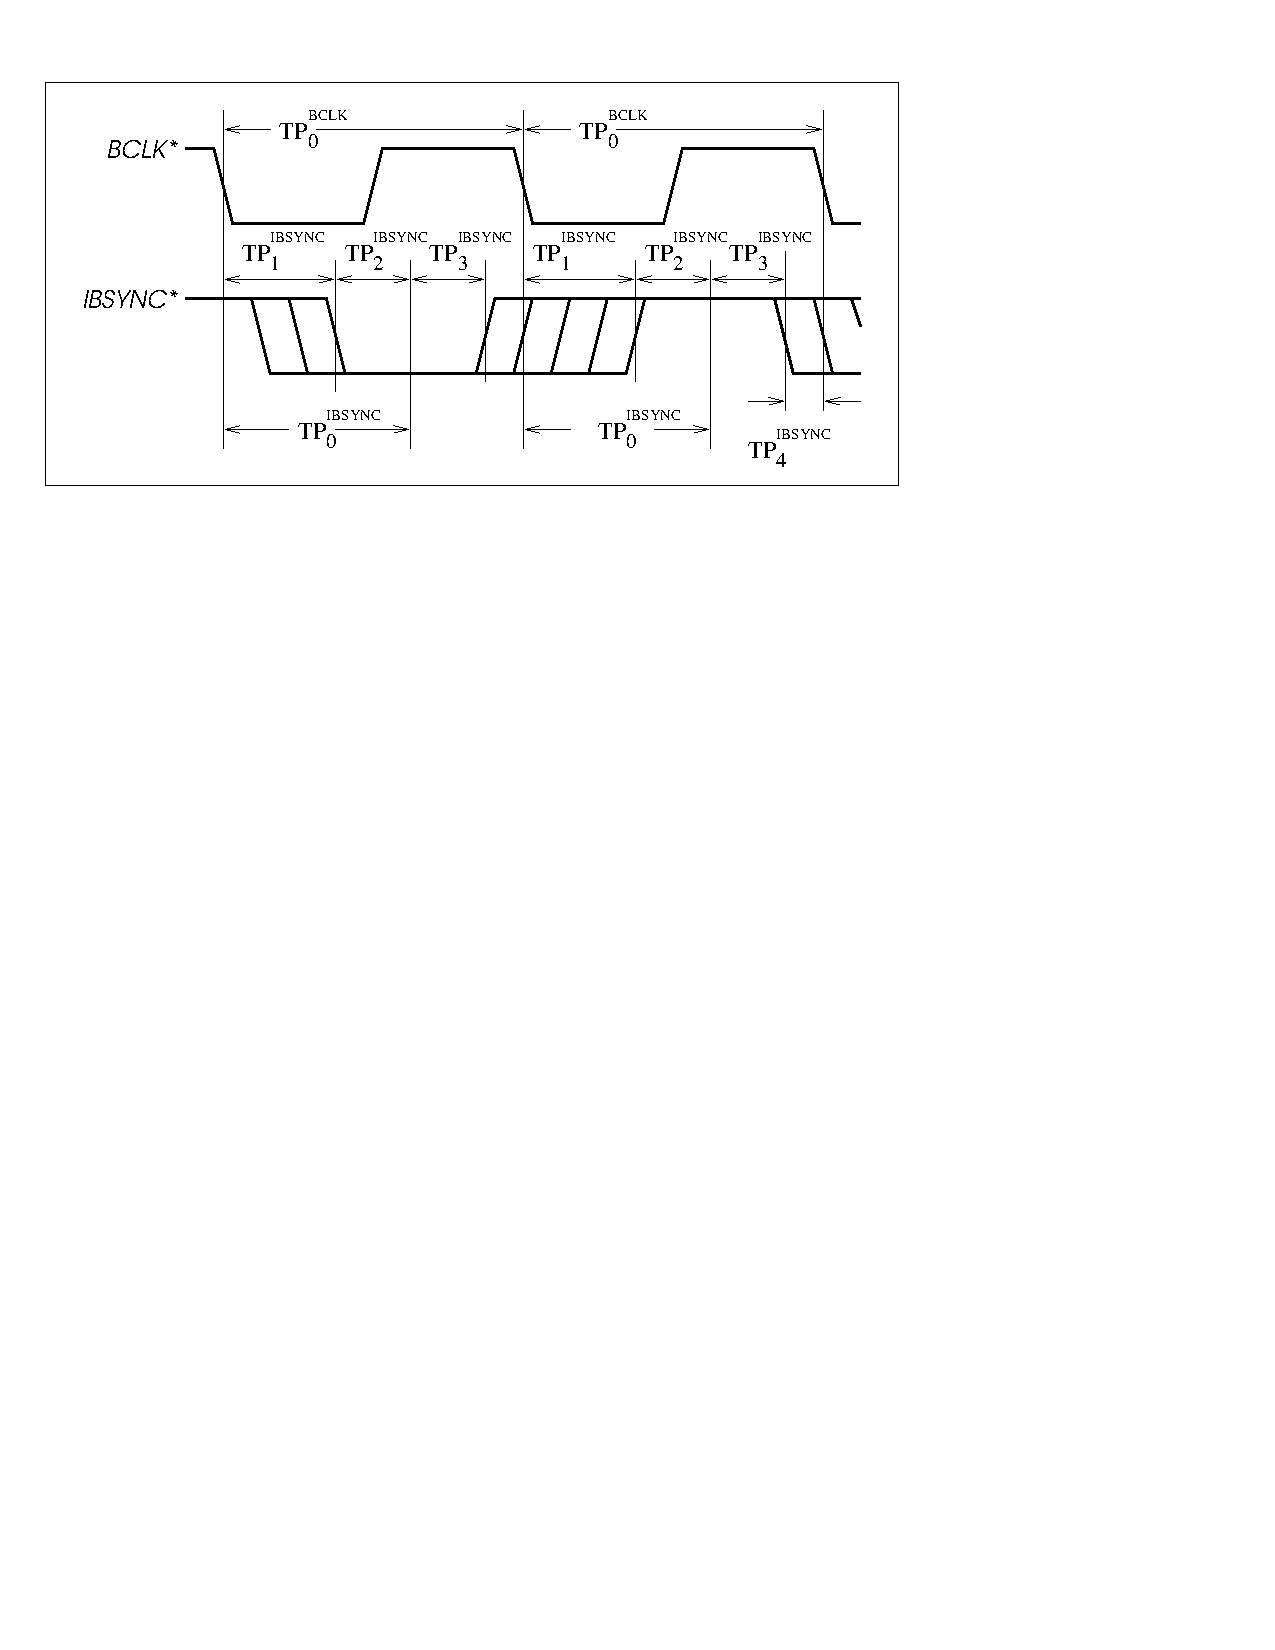
\includegraphics{ch6/FIG/ibsync-time.jpg}}
   \caption{IBSYNC* 신호의 시간규격}\label{figure:ibsync-time}
\end{figure}
%
%
\subsection{인터럽트 버스 중재 동작의 시간 규격}
중재 주기는 버스 클럭 (BCLK*)의 하강점부터 시작되며,
$TP^{IBARB}_0 + TP^{IBARB}_1$동안 신호를 구동해야 한다.
특히 중재결과는 $TP^{IBARB}_0$ 시점에 래치할 수 있도록 안정된 신호를
보장해야 한다.
%\documentstyle[a4]{hbook}
%\begin{document}
%
\begin{table}[htbp]
\caption{인터럽트 중재 버스 신호의 시간규격 요약}\label{table:ibarb-time}
   \begin{center}
   \begin{tabular}{|l|l|r|r|r|} \hline
	timing parameter & name & min & typical & max \\ \hline \hline
	$TP^{BCLK}_0$  & BCLK* cycle time & 59 & 60 & 61 \\ \hline
	$TP^{IBARB}_0$  & arbitration time & 240 & 242 & 244 \\ \hline
	$TP^{IBARB}_1$  & post time & 20 & 30 & 40 \\ \hline
	$TP^{IBARB}_2$  & guard time & 10 & - & - \\ \hline
   \end{tabular}
   \end{center}
\end{table}
%
%\end{document}

\begin{figure}[htb]
    \centerline{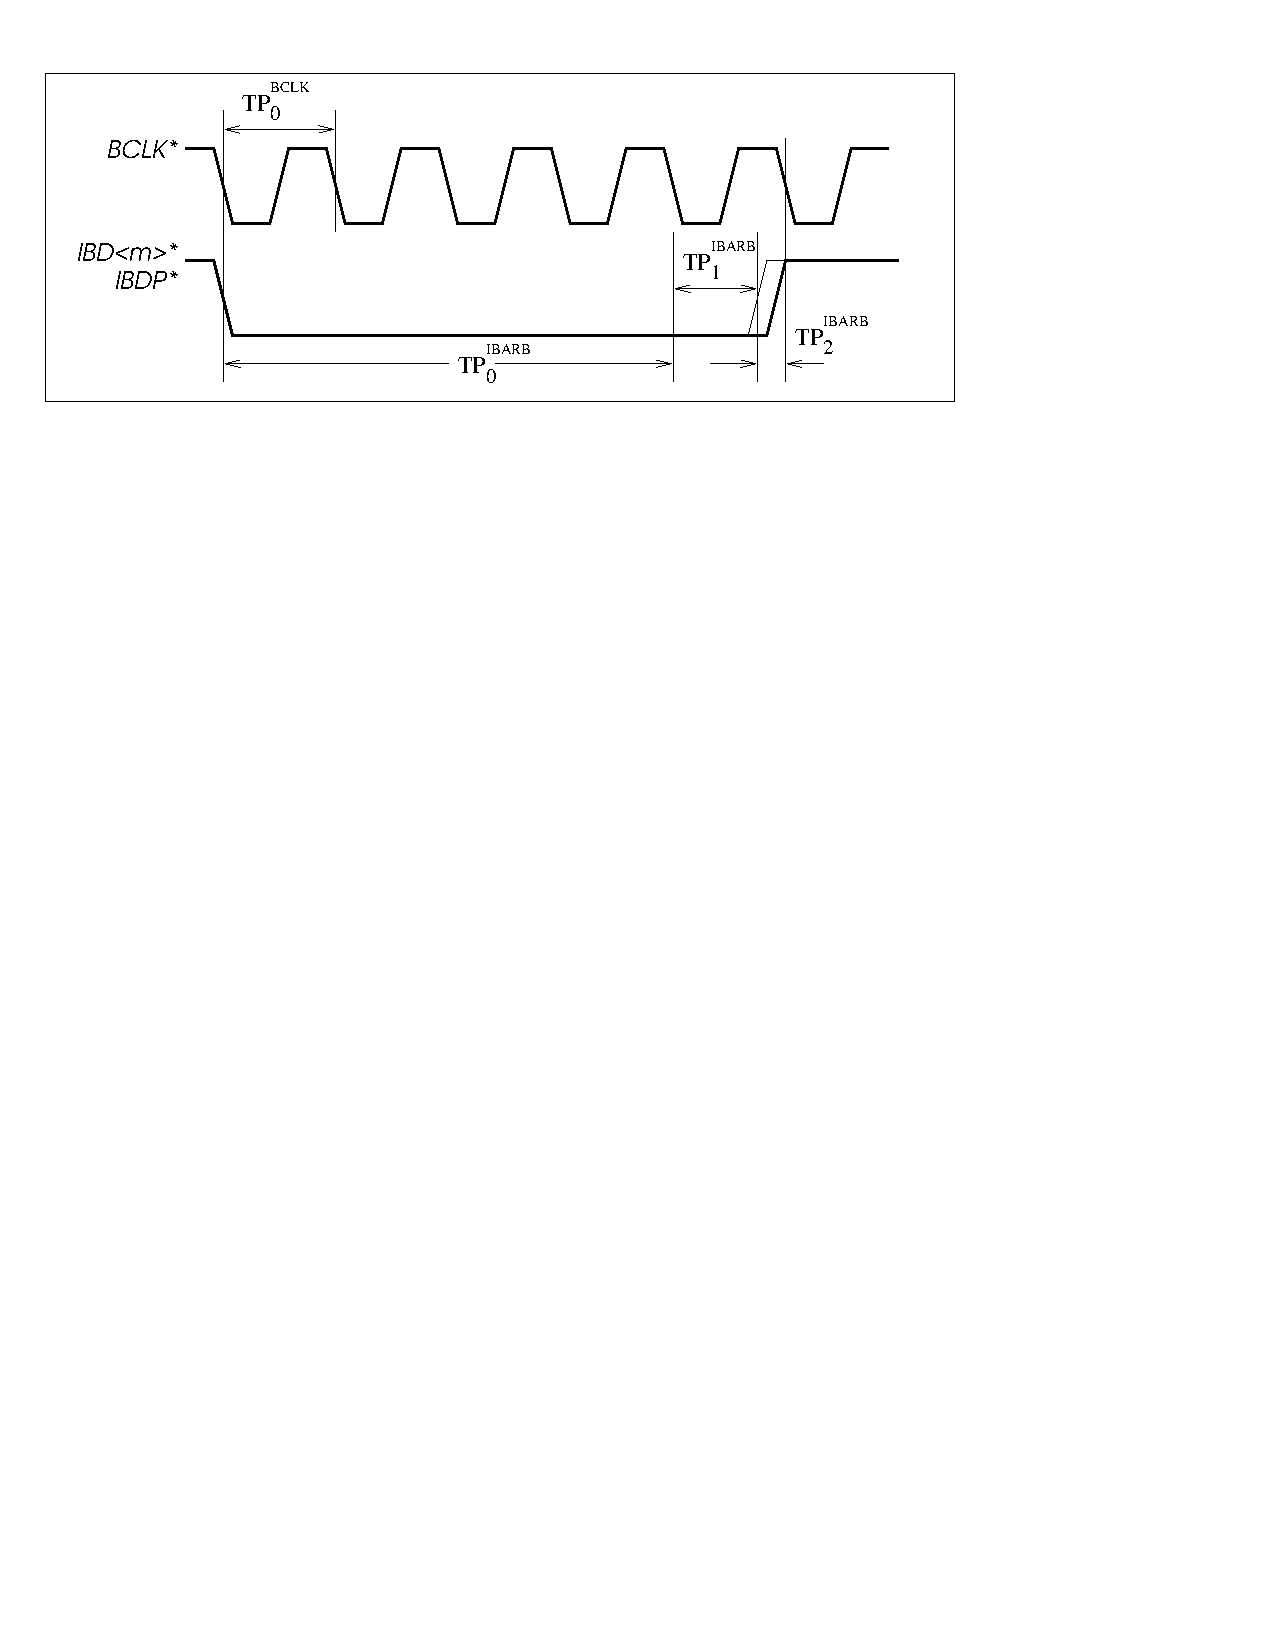
\includegraphics{ch6/FIG/ibarb-time.jpg}}
   \caption{인터럽트 버스 중재 동작의 시간규격}\label{figure:ibarb-time}
\end{figure}
%
\subsection{인터럽트 버스 인터럽트 데이터 전송 주기의 시간 규격}
인터럽트 버스를 통하여 전송하고자 하는 데이터의 신호는
백플레인에 나타나는 버스클럭의 하강점에서 $TP^{IBD}_0$ 후에
안정된 신호를 래치할 수 있도록 셋업시간으로 $TP^{IBD}_2$을
홀드시간으로 $TP^{IBD}_3$를 보장하여야 한다.
그리고 앞과 뒤 신호에 영향을 주지 않도록 $TP^{IBSYNC}_4$을
보장하여야 한다.
%
%\documentstyle[a4]{hbook}
%\begin{document}
%
\begin{table}[htbp]
\caption{인터럽트 버스의 인터럽트 데이터 신호의 시간규격 요약}\label{table:ibd-time}
   \begin{center}
   \begin{tabular}{|l|l|r|r|r|} \hline
	timing parameter & name & min & typical & max \\ \hline \hline
	$TP^{BCLK}_0$ & BCLK* cycle time & 59 & 60 & 61 \\ \hline
	$TP^{IBD}_0$  & IBD{\tt <}n{\tt >}* signal latch point & 38 & 40 & 42 \\ \hline
	$TP^{IBD}_1$  & bus propagation time & - & - & 20 \\ \hline
	$TP^{IBD}_2$  & setup time & 10 & - & - \\ \hline
	$TP^{IBD}_3$  & hold time & 5 & - & - \\ \hline
	$TP^{IBD}_4$  & guard time & 10 & - & - \\ \hline
   \end{tabular}
   \end{center}
\end{table}
%
%\end{document}

\begin{figure}[htb]
    \centerline{\includegraphics{ch6/FIG/ibd-time.jpg}}
   \caption{인터럽트 버스의 데이터 전송의 시간규격}\label{figure:ibd-time}
\end{figure}
%%%
